\documentclass[a4paper,11pt,oneside]{report}
\usepackage[top=2.2cm, bottom=2cm, left=2.3cm, right=2cm]{geometry}
\usepackage{graphicx}
\usepackage{titlesec}
\usepackage{fvextra}
\usepackage{minted}
\usepackage{amsmath}
\usepackage{amssymb}
\usepackage{xcolor}
\usepackage{tocloft}
\usepackage{caption}
\usepackage{cite}
\usepackage[nottoc,notlof,notlot]{tocbibind}
\usepackage{float}
\usepackage{array}
\usepackage{booktabs}
\usepackage{tikz}
\usepackage{url}
\usepackage[hidelinks,plainpages=false,pdfpagelabels]{hyperref}
\setlength{\emergencystretch}{3em}
\usetikzlibrary{positioning,arrows.meta,shapes.geometric,shapes.misc,calc}

% ---------- flowchart styles ----------
\tikzset{
  term/.style={rounded rectangle, draw=black, align=center, font=\small,
               inner sep=3pt, minimum height=0.7cm, text width=6.2cm},
  block/.style={rectangle, draw=black, align=center, font=\small,
                inner sep=3pt, minimum height=0.7cm, text width=7.2cm},
  dec/.style={diamond, draw=black, aspect=3.2, align=center, font=\small,
              inner sep=1pt, text width=3.2cm},
  arr/.style={-{Stealth[length=2mm]}, thick}
}

% ---------- minted defaults ----------
\setminted{style=tango, linenos, breaklines, autogobble, fontsize=\scriptsize,
           frame=lines, framesep=1mm, numbersep=6pt}
% \srcexcerpt{first line}{last line}  -> lines of code/main.cpp, original line numbers kept
\newcommand{\srcexcerpt}[2]{%
  \inputminted[firstline=#1,lastline=#2,firstnumber=#1]{cpp}{code/main.cpp}}
\newcommand{\srccaption}[1]{\par\smallskip\noindent\textbf{\small #1}\par\nobreak}

% ---------- chapter formatting ----------
\titleformat{\chapter}[display]
  {\normalfont\bfseries\LARGE}
  {\chaptertitlename\ \thechapter}
  {4pt}
  {}
\titlespacing{\chapter}{0pt}{-25pt}{12pt}
\renewcommand{\bibname}{References}
\renewcommand{\contentsname}{Table of Contents}
\captionsetup{font=small,labelfont=bf}

% ---------- metadata ----------
\newcommand{\studentname}{Sadman Ishtiak}
\newcommand{\course}{CSE-428: Computer Graphics Lab}
\newcommand{\institute}{Jatiya Kabi Kazi Nazrul Islam University}
\newcommand{\supervisor}{Dr. Habiba Sultana}
\newcommand{\supervisordesignation}{Associate Professor}
\newcommand{\studentdetails}{Session: 2021--22\\ Roll: 22102009 \\ Reg: 10815}
\newcommand{\reportdate}{November 15, 2026}
\title{Maze Runner 3D}
\author{\studentname}
\date{\reportdate}

\let\cleardoublepage\clearpage
\begin{document}

% ---------- title page ----------
\begin{titlepage}
  \centering
  
\includegraphics[width=0.2\textwidth]{images/Jatiya_Kabi_Kazi_Nazrul_Islam_University_Logo.png}\\[0.4cm]
  {\LARGE\bfseries \institute}\\[3pt]
  {\large Trishal, Mymensingh}\\[0.5cm]
  {\Large\bfseries Department of Computer Science and Engineering}
  \vfill
  {\Large Technical Report on}\\[0.3cm]
  {\Huge\bfseries Maze Runner 3D}\\[0.3cm]
  {\large}\\[0.5cm]
  {\LARGE\bfseries \course}
  \vfill
  {\Large\bfseries Submitted To}\\[0.2cm]
  {\Large \supervisor}\\
  {\large \supervisordesignation}\\
  {\large Department of Computer Science and Engineering}\\
  {\large \institute}
  \vfill
  {\Large\bfseries Submitted By}\\[0.2cm]
  {\Large \studentname}\\
  {\large \studentdetails}
  \vfill
  {\large Submission Date: \reportdate}
\end{titlepage}

% ---------- front matter ----------
\pagenumbering{Roman}
\setcounter{secnumdepth}{2}
\setcounter{tocdepth}{1}
\tableofcontents
\clearpage
\pagenumbering{arabic}

% ---------- chapters ----------
\chapter{Introduction}

Most 3D games today lean on the GPU to draw triangles, but there is a much older and simpler way to put a 3D world on the screen: ray casting. For every pixel you send a ray out from the eye, find the first surface it hits, and colour the pixel accordingly. When the world is built on a regular grid, like the walls of a maze, finding that first surface is cheap, because you only need to step from one grid cell to the next along the ray. I wanted to see how far this idea could go on its own, so I built a small first-person maze game around it.
\\

Maze Runner 3D is written in C++20 as a single file, \texttt{main.cpp}, and every pixel is computed on the CPU. SDL2 is used only to open a window, show the finished image and read the keyboard; there are no shaders and no image files. The vector and ray classes follow the style of \emph{Ray Tracing in One Weekend}~\cite{shirley_rtiow}, the window set-up follows the SDL documentation~\cite{sdlwiki}, and walls are found with the grid-walking method of Amanatides and Woo~\cite{amanatides1987fast}.
\\

The player starts at the \texttt{S} of a $16\times16$ maze and has to reach the \texttt{E}, which appears as a bright green tile on the floor. You move with \texttt{W}/\texttt{S} or the arrow keys, strafe with \texttt{A}/\texttt{D}, turn with the left and right arrows, and hold Shift (or turn on Caps Lock) to sprint. The walls are solid, so you cannot walk through them, but you slide along them instead of getting stuck. The scene is lit by a light that travels with the player, and a ``hot/cold'' score, shown in the window title and as a colour bar at the top of the screen, tells you how close you are to the exit by the actual walking distance rather than the straight line.
\\

This report explains how the program works. The next chapter covers the geometry and algorithms behind the renderer, the movement and the score, the third chapter walks through the code, the fourth shows the output, and the last discusses the limitations I noticed and concludes. The excerpts keep the line numbers of the original \texttt{main.cpp}.

\chapter{Methodology}

% Code excerpts below are taken directly from \texttt{main.cpp}; the line numbers beside them are the file's own.

\section{World and Map}

The world is right-handed with $z$ up: $x,y$ span the ground, the floor is $z=0$, walls are unit cubes with $z\in[0,\texttt{WALL\_H}]$, $\texttt{WALL\_H}=1$, the ceiling is $z=1$, and the eye stays at $z=\texttt{EYE\_HEIGHT}=0.5$.

The maze is the array \texttt{MAP[16]} of 16-character strings (lines 9--26), with \texttt{\#} for wall, \texttt{.} for floor, \texttt{S} for the start and \texttt{E} for the exit. \texttt{MAP[cy][cx]} is the cell whose ground square is $[c_x,c_x+1]\times[c_y,c_y+1]$, so the row index is world $y$ (the code names it \texttt{start\_z}/\texttt{exit\_z} in places, but it is always used as $y$). \texttt{is\_wall} treats everything outside the map as solid, so neither rays nor the player can leave it.

\section{Camera Model}

The camera is a pinhole at the eye position $\mathbf{O}=(x,y,0.5)$ with a single orientation angle, the yaw $\psi$ (no pitch or roll). The basis is
\begin{equation}
\mathbf{F}=(\cos\psi,\sin\psi,0),\quad \mathbf{U}=(0,0,1),\quad \mathbf{R}=\mathbf{F}\times\mathbf{U}=(\sin\psi,-\cos\psi,0).
\end{equation}
An image plane at distance 1 has half-width $h_w=\tan(\mathrm{FOV}/2)\approx0.767$ and half-height $h_h=h_w H/W\approx0.576$, with $\mathrm{FOV}=75^\circ$ and $W\times H=640\times480$. For pixel $(i,j)$,
\begin{equation}
u_i=\Big(\tfrac{2(i+0.5)}{W}-1\Big)h_w,\quad
v_j=\Big(1-\tfrac{2(j+0.5)}{H}\Big)h_h,\quad
\mathbf{D}_{ij}=\frac{\mathbf{F}+u_i\mathbf{R}+v_j\mathbf{U}}{\lVert\mathbf{F}+u_i\mathbf{R}+v_j\mathbf{U}\rVert},
\end{equation}
and the ray is $\mathbf{P}(t)=\mathbf{O}+t\mathbf{D}_{ij}$. Because $\mathbf{D}$ is a unit vector, $t$ is the true distance from the eye.

\srcexcerpt{262}{284}

The basis depends only on yaw, so it is computed once per frame outside the pixel loops. Colours in $[0,1]$ are packed into 32-bit ARGB; multiplying by $255.99$ before truncating maps $1.0$ to $255$.

\section{Ray--Surface Intersection}

\texttt{cast\_ray} (lines 164--225) returns a \texttt{hit\_record} (distance, point, normal, colour), starting from $t=10^{30}$ meaning ``no hit''.

\textbf{Floor and ceiling.} A plane $z=z_p$ is met at $t=(z_p-O_z)/D_z$. Rays pointing down ($D_z<-10^{-9}$) can only hit the floor, rays pointing up only the ceiling, and near-horizontal rays skip both, which avoids division by almost zero. The floor colour comes from \texttt{floor\_color\_at}: bright green inside the exit cell, otherwise light or dark grey by the parity of $\lfloor x\rfloor+\lfloor y\rfloor$ (a checkerboard). The distance \texttt{t\_plane} is kept; a wall only matters if it is nearer.

\textbf{Walls: grid traversal.} With $(c_x,c_y)$ the eye's cell and $s_x,s_y\in\{\pm1\}$ the signs of $D_x,D_y$, the distance along the ray needed to cross one cell is $\Delta t_x=|1/D_x|$, $\Delta t_y=|1/D_y|$, and the first grid-line crossings are
\begin{equation}
t_x=\begin{cases}(c_x+1-O_x)\Delta t_x & s_x>0\\ (O_x-c_x)\Delta t_x & s_x<0\end{cases}\qquad
t_y=\begin{cases}(c_y+1-O_y)\Delta t_y & s_y>0\\ (O_y-c_y)\Delta t_y & s_y<0.\end{cases}
\end{equation}
At each step the smaller of $t_x,t_y$ is the next grid line crossed: it becomes the entry distance $t_{\text{entry}}$, the cell index moves by $s_x$ or $s_y$, and that value grows by $\Delta t_x$ or $\Delta t_y$. Cells are therefore visited in the exact order the ray passes through them. On entering a wall cell, the ray's altitude $O_z+t_{\text{entry}}D_z$ is checked against $[0,\texttt{WALL\_H}]$; if inside, the face just crossed is the visible surface, with normal $(-s_x,0,0)$ or $(0,-s_y,0)$, and the function returns immediately since the first hit is the nearest. The loop is capped at 256 steps and stops once $t_{\text{entry}}$ passes \texttt{t\_plane}.

\srcexcerpt{187}{225}

\section{Shading}

A single point light sits at the eye, like a torch carried by the player, so every visible point is lit and no shadow rays are needed. With surface normal $\mathbf{N}$, unit vector $\boldsymbol\ell$ to the eye, squared distance $d^2$ and material colour $\mathbf{k}$:
\begin{equation}
\mathbf{C}=\mathbf{k}\odot\Big(\mathbf{a}+\mathbf{L}\max(\mathbf{N}\!\cdot\!\boldsymbol\ell,0)\tfrac{1}{0.9+0.30d^2}\Big),\qquad C'_c=\sqrt{\operatorname{clamp}(C_c,0,1)},
\end{equation}
with ambient $\mathbf{a}=(0.14,0.14,0.18)$ and torch colour $\mathbf{L}=(1.7,1.45,1.10)$. The square root is a gamma of 2.0, approximating a display's nonlinear response. Material colours are tan $(0.55,0.47,0.40)$ for walls, $(0.22,0.22,0.26)$ for the ceiling, $(0.60,0.58,0.55)$ and $(0.30,0.30,0.33)$ for floor tiles, and $(0.20,0.85,0.30)$ for the exit tile.

\srcexcerpt{227}{239}

\section{Movement and Collision}

\texttt{update} (lines 286--316) converts key states into signed inputs: yaw changes by $\pm\texttt{TURN\_SPD}\,\Delta t$ ($2.5$ rad/s), forward is the sum of \texttt{W}/Up minus \texttt{S}/Down clamped to $[-1,1]$, and strafe is \texttt{D} minus \texttt{A}. The ground step is $(f\mathbf{F}+g\mathbf{R})\,v\,\Delta t$ with $v=2.0$ units/s, or $5.0$ while sprinting. Diagonal input is not normalised, so it is $\sqrt2$ times faster.

Since the eye is always inside the wall height range, collision is two-dimensional: the player is a circle of radius $0.28$ against unit squares. For each wall cell overlapping the circle's bounding box, the closest point $q$ of the square to the centre $p$ is found by clamping, and a collision occurs if $\lVert p-q\rVert^2<0.28^2$ (no square root needed). The $x$ and $y$ parts of each step are tested and applied separately, so a blocked component is dropped and the player slides along the wall.

\srcexcerpt{241}{260}

\section{Hot/Cold Score}

A straight-line distance would mislead in a maze, so a breadth-first search (BFS) starts at the exit and expands over floor cells in four directions, storing in \texttt{exit\_dist} the walking distance of every cell. It runs once, before the main loop (lines 59--74).

\srcexcerpt{59}{74}

With $d$ the distance of the player's cell and $d_{\max}$ the largest distance, the score is $T=1-2d/d_{\max}\in[-1,1]$: $+1$ on the exit, $-1$ in the farthest cell. Labels are \texttt{HOT} for $T>0.5$, \texttt{WARM} for $T>0$, \texttt{COOL} for $T>-0.5$, otherwise \texttt{COLD}.

\chapter{Implementation}

\section{Program Structure}

\begin{table}[H]
\centering
\caption{Structure of \texttt{main.cpp} (459 lines)}
\label{tab:funcs}
\small
\begin{tabular}{@{}p{4.4cm}p{1.8cm}p{8.2cm}@{}}
\toprule
\textbf{Part} & \textbf{Lines} & \textbf{Purpose} \\
\midrule
Includes, \texttt{MAP}, constants & 1--41 & Maze data and tunable parameters \\
\texttt{is\_wall}, \texttt{build\_exit\_dist} & 43--74 & Solid-cell test; BFS distance from the exit \\
\texttt{vec3}, \texttt{ray}, \texttt{hit\_record} & 76--136 & Vector maths and intersection result \\
\texttt{temperature}, \texttt{floor\_color\_at} & 138--162 & Score in $[-1,1]$; checkerboard and exit tile \\
\texttt{cast\_ray}, \texttt{shade} & 164--239 & Intersection and lighting \\
\texttt{collides} & 241--260 & Circle-versus-wall test \\
\texttt{render} & 262--284 & One frame into the pixel buffer \\
\texttt{update} & 286--316 & Input, movement, wall sliding \\
\texttt{main} & 319--459 & SDL set-up, game loop, clean-up \\
\bottomrule
\end{tabular}
\end{table}

\section{Code}

\srccaption{Constants (lines 30--41)}
\srcexcerpt{30}{41}

\srccaption{Window, renderer and texture set-up (lines 320--369)}
\srcexcerpt{320}{369}

\srccaption{Finding \texttt{S} and \texttt{E}, spawning the player (lines 371--385)}
\srcexcerpt{371}{385}

\srccaption{Main loop (lines 387--448)}
\srcexcerpt{387}{448}

\srccaption{Shutdown (lines 450--459)}
\srcexcerpt{450}{459}

\chapter{Results and Evaluation}

\section{Rendered Output}

Figure~\ref{fig:views} shows frames produced by the program's own rendering code (lines 1--316 of \texttt{main.cpp}, unmodified, compiled into a small test program that writes the $640\times480$ pixel buffer to an image). They show the 3D view only; the window title and hot/cold bar are drawn by SDL in \texttt{main} and are not included.

\begin{figure}[H]
\centering
\begin{minipage}{0.32\textwidth}\centering
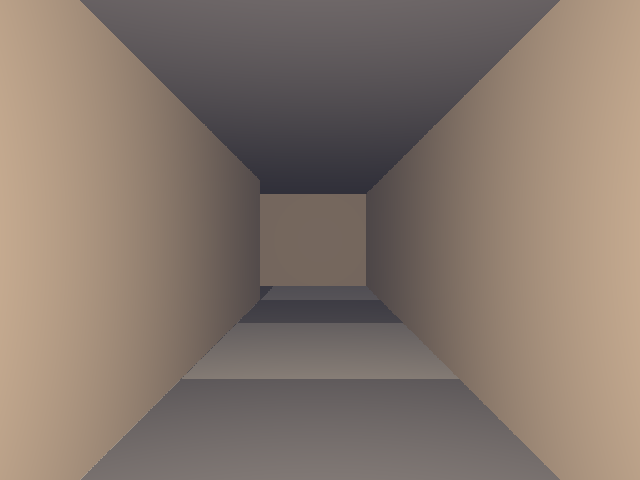
\includegraphics[width=\linewidth]{images/view_spawn.png}\\[2pt]{\small (a)}
\end{minipage}\hfill
\begin{minipage}{0.32\textwidth}\centering
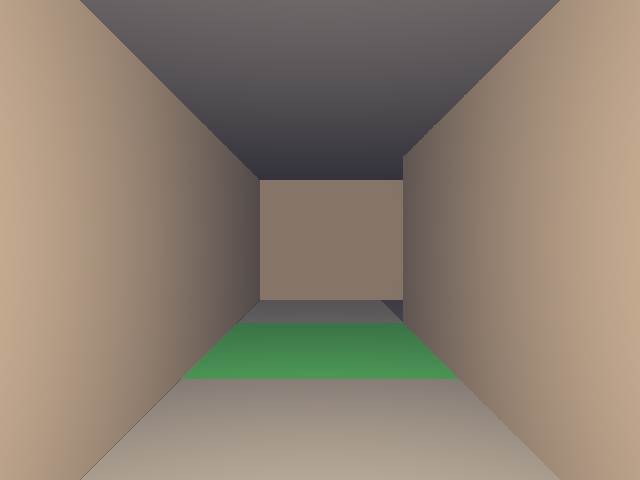
\includegraphics[width=\linewidth]{images/view_exit.png}\\[2pt]{\small (b)}
\end{minipage}\hfill
\begin{minipage}{0.32\textwidth}\centering
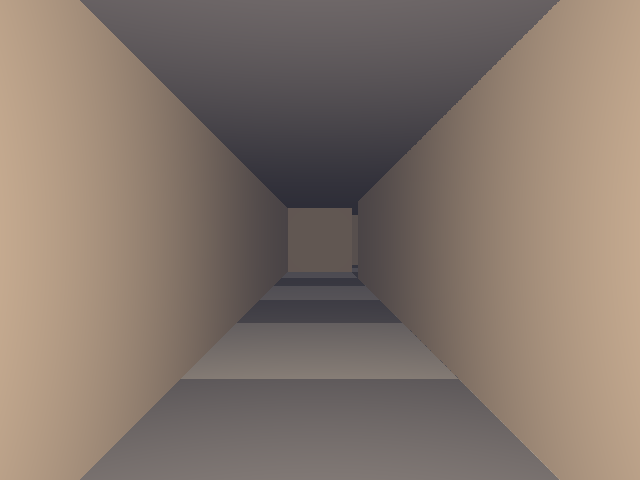
\includegraphics[width=\linewidth]{images/view_checker.png}\\[2pt]{\small (c)}
\end{minipage}
\caption{Rendered frames. (a) Spawn position $(1.5,1.5)$ facing $+x$. (b) From $(4.5,9.5)$ facing $+x$: the green exit tile ahead. (c) From $(9.5,13.5)$ facing $-x$: alternating floor tiles.}
\label{fig:views}
\end{figure}

The images show perspective convergence of the corridors and correct occlusion (the grid walk returns the first wall entered); torch lighting that brightens near surfaces and fades with distance; a green tile only on the exit cell with grey neighbours; and a checkerboard floor.

\section{Collision and Performance}

Calling \texttt{collides} on the unmodified code gave: free at the spawn $(1.5,1.5)$; blocked inside the border wall $(0.5,0.5)$; blocked at $(1.5,1.2)$, which is $0.2$ from the wall and less than the radius $0.28$; and free at $(1.5,1.3)$, $0.3$ from the wall. All four match the expected result.

Each frame casts $640\times480=307{,}200$ rays. Calling \texttt{render} 30 times on one thread with \texttt{-O3} took about 11--12~ms per frame (roughly 85 frames/s) on the machine used to prepare this report; the value depends on the processor. In the game, a frame is padded to at least about 15~ms and presentation is vsynced when available, so the displayed rate is limited to about 60--66 frames/s.

\chapter{Limitations and Conclusion}

\section{Limitations}

These points come from reading the source:
\begin{enumerate}
    \item \textbf{Mirrored view.} The camera's right vector is $(\sin\psi,-\cos\psi,0)$ while the map row index is used as $y$ and increases downward on the page, so the rendered maze is the mirror image of how \texttt{MAP} is written. The game stays consistent and solvable.
    \item \textbf{Debug output.} Line 407 prints \texttt{dt} to the console every frame, before the clamp.
    \item \textbf{Diagonal speed.} Forward and strafe input are not normalised together, so diagonal movement is $\sqrt2$ times faster.
    \item \textbf{Plain materials and one thread.} Walls and ceiling are single colours with no textures, and all rays are traced on one thread.
    \item \textbf{Fixed maze, abrupt ending.} There is one built-in maze, and reaching the exit only prints a message and closes the window.
    \item \textbf{Portability.} \texttt{<bits/stdc++.h>} is a GCC header.
\end{enumerate}
Natural next steps are removing the debug print, normalising movement, splitting the image into bands for several threads, adding wall textures, and loading or generating mazes.

\section{Conclusion}

Maze Runner 3D renders a convincing first-person maze entirely on the CPU: unit rays from a pinhole camera, analytic floor and ceiling planes, a grid walk that returns the nearest wall, torch lighting with gamma encoding, circle-versus-square collision with wall sliding, and a breadth-first-search distance field that drives the hot/cold score. All objectives were met in 459 lines with SDL2 used only for display and input. The project shows that for grid-aligned scenes, ray casting needs no acceleration structures, shaders or image assets, and that the same grid also makes collision and shortest-distance computation short and exact.


% ---------- references ----------
\clearpage
\bibliographystyle{ieeetr}
\bibliography{reference/reference}

\end{document}
